\documentclass[11pt]{article}

\usepackage{graphics} % or graphicx 
\usepackage{epstopdf}
\usepackage{multirow}
\usepackage{amsmath}
\usepackage{bbding}
\usepackage{pifont}
\usepackage{wasysym}
\usepackage{amssymb}
\usepackage{subcaption}
\usepackage{verbatim}


\setlength{\oddsidemargin}{0in}
\setlength{\textwidth}{6.5in}
\setlength{\topmargin}{-0.5in}
\setlength{\textheight}{8.75in}
\setlength{\parindent}{0pt}
\setlength{\parskip}{6pt}

\usepackage{fancyhdr}
\pagestyle{fancy}
\lhead{HW7} %----------------------------------------------------------- change
\rhead{Reza Shisheie}

\usepackage{epsfig,graphicx}

\usepackage{amsmath}

\usepackage{clrscode3e}

\begin{document}

\thispagestyle{plain}

\begin{center}
{\Large \bf CIS 606 \hfil Homework 7 \hfil Fall 2019} \\%--------------- change
\end{center}

\vskip 1in 

\centerline{\includegraphics[width=3in]{photo.jpg}}

\vskip 0.5in 


\begin{center}
\begin{tabular}{ll}
{\bf Name:}     & {\bf Reza Shisheie } \\ \\
{\bf Login ID:} & {\bf reshishe }   
\end{tabular}
\end{center}

\newpage

\begin{enumerate}

\itemsep 0.35in



\item Give an integer length $x$, and the integer cutting points $x_1,x_2,...,x_n$ (where $1 \leq x_i \leq x$ for $1\leq i \leq n$), find the minimum cost of cutting a piece of iron bar of length $x$ at the $n$ points at distance $x_1,x_2,...,x_n$ from the left-hand end (given that cutting a piece of bar of length $y$ at any cost $y$). Devise a polynomial -time algorithm for the problem using dynamic programing technique.  
	
	The solution to this problem is based on the location of cut. The bar starts at position $l=0$ which is denoted by $l_0$ and ends at position $l=L$ which is full length  and is denoted by $l_n$. 
	
	A visual diagram of the bar with cuts is shown in Figure.\ref{fig:bar_partition}.
        
    \begin{figure}[h!]
		\centerline{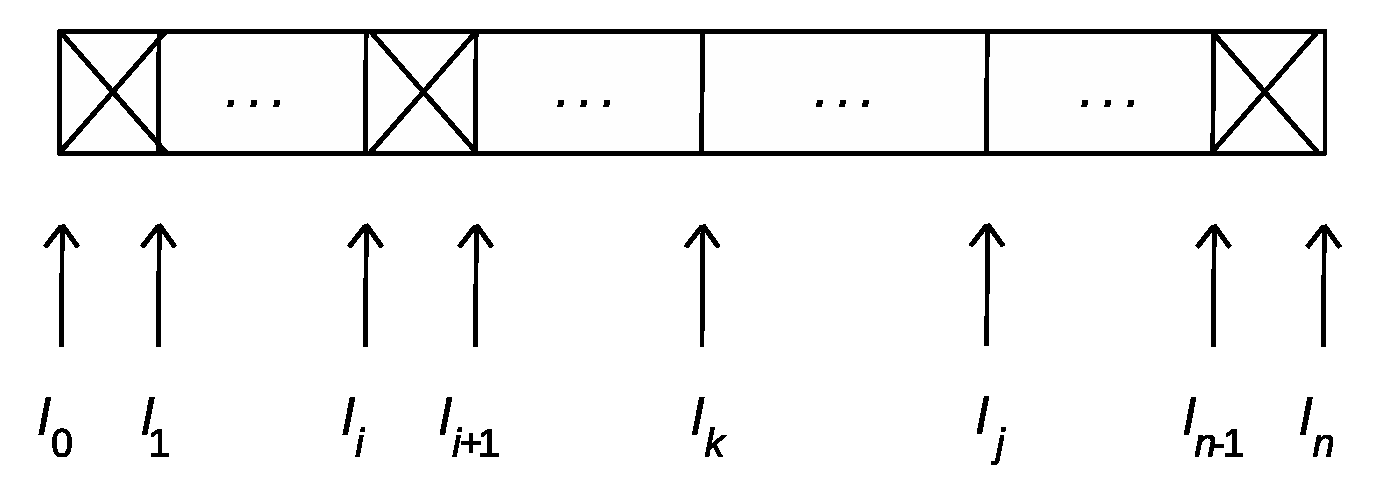
\includegraphics[width=4in]{bar_partition.eps}}
		\caption{Cutting points. It starts from 0 and cuts through the bar to $n$}
		\label{fig:bar_partition}
	\end{figure}
	
	Cutting points for a piece of rod which starts at position $l_i$ and ends at position $l_j$ is located at $l_k$. Therefore $i<k<j$. 
	
	Let $m[i,j]$ be dynamic variable which is the minimum cost of cuts from point $i$ o point $j$.
	
	\begin{equation}
	m[i,j] =
    	\begin{cases}
      	0 & \text{if $j-i=0$ or $j-i=1$}\\
      	m[i,k]+m[k,j]+l_j-l_i & \text{otherwise}
    	\end{cases}       
	\end{equation}
	
	where $l_j-l_i$ is the length of rod from position $i$ to $j$. 
	
	
\pagebreak
	
	Two algorithms are provided to find optimal cut and then print where cuts should take place. 	
	
	First algorithm $-\proc{Min-Cost-Cut}(L,c,l)-$ finds the most optimal cut, where $L$ is the full length of the rod, $c$ is the number of cuts, and $l$ is the location of cuts. 
	
	The Second algoritgm $-\proc{Min-Cost-Cut}(L,c,l)-$, prints the precedence of cuts. 
	
	
	\begin{codebox}
		\Procname{$\proc{Min-Cost-Cut}(L,c,l)$}
		
		\li \Comment Reeconstruct $l$ by adding $l_0=0$ and $l_n=L$ to the beginning and end of $l$ 
		\li $l=[0,[l],l_n]$
		\li \Comment $n$ is the maximum number of pieces, which is number of cuts$+1$.
		\li $n=c+1$
		
		\li \Comment generate matrix $m$ to accumulate cost and matrix $s$ to store location of cut and initilize to 0.
		\li $m=\mathrm{zero}(n\times n)$
		\li $s=\mathrm{zero}(n\times n)$
		
		\li \For $l_c=2 \rightarrow n$
		\Do	
		\li 	\For $i=0 \rightarrow n-l_c$
		\li 	\Do
					$j=i+l_c$
		\li			$m[i,j]=\infty$
		\li 		\For $k=i+1 \rightarrow j-1$
		\li 		\Do
						$q=m[i,k]+m[k,j]+l_j-l_i$
		\li				$m[i,j]=\infty$
		\li 			\If $q<m[i,j]$
		\li 			\Do	
			                $m[i,j]=q$
		\li	                $s[i,j]=k$

						\End

					\End

				\End
			\End
		\li print($m[0,n]$)
		\li $\proc{Print-Cut}(l,s,i,j)$
		
	\end{codebox}
	
	Time complexity of $\proc{Min-Cost-Cut}(L,c,l)$ is $O(n^3)$ since it has 3 internal loops. It is actually almost identical to the matrix multiplication time complexity. 

	\begin{codebox}
		\Procname{$\proc{Print-Cut}(l,s,i,j)$}
		
		\li \Comment if bar length is 2, then just return where the cut last cut is. This is the minimum cutable piece  
		\li \If $(j-i)=2$
		\li		\Do
					return print($l_{s[i,j]}$) 
				\End
		\li \Comment if bar length is 1 or 0, return nothing. Bar is not cuttable. 
		\li \ElseIf $(j-i)=1$ or $i=j$
		\li		\Do
					return $\emptyset$ 
				
		\li \Comment if bar length is larger than 2, then print where the last cut is and then cut the left and right sides
		\li \Else 
		\li		\Do
			 		print($l_{s[i,j]}$)				
		\li			$\proc{Print-Cut}(l,s,i,s[i,j])$
		\li			$\proc{Print-Cut}(l,s,s[i,j],j)$ 
				\End
		
	\end{codebox}

\pagebreak

	
\item Write a program in Python 3 to solve previous problem. 

	A snippet of code is hown in Figure\ref{fig:python_code}. Notice the uses uses $"numpy"$ library.
	
	\begin{figure}[h!]
		\centerline{\includegraphics[width=5.5in]{python_code.png}}
		\caption{Snippet of code}
		\label{fig:python_code}
	\end{figure}

	\pagebreak
	

	Cheapest cut costs 73 and the precedence of cuts are:
	
	$[13, 5, 24, 17] $ which is $13 \rightarrow 5 \rightarrow 24 \rightarrow 17 $
	

	\begin{figure}[h!]
		\centerline{\includegraphics[width=6in]{result.png}}
		\caption{Results}
		\label{fig:result}
	\end{figure}
	 

	This is how cuts happen:
	
	\begin{figure}[h!]
		\centerline{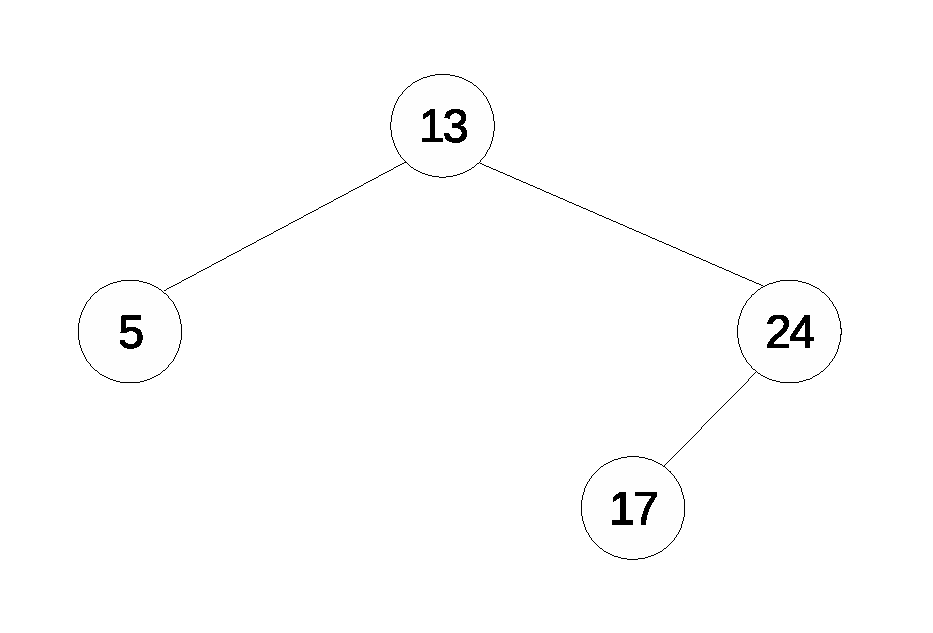
\includegraphics[width=4in]{cuts.eps}}
		\caption{Precedence of cuts}
		\label{fig:cuts}
	\end{figure}

	









	
	
	
	
	
	





































   
\end{enumerate}

\end{document}

